%************************************************************************************
% Authors: Martin Nordio
% Date: March 2011
% Root file: report_root.tex
%************************************************************************************


%----------------------------------------------------------------------------
\chapter{Design}\label{design}
%----------------------------------------------------------------------------


\section{Introduction}


The following subsections discuss the features that I want CloudStudio to provide and how these features can greatly improve the collaboration experience for users, as well as the approach behind the implementation of CloudStudio.


\subsection{Features}\label{designfeatures}

CloudStudio provides numerous awareness and conflict detection features that users can benefit from. The following is a list of provided awareness information:


\begin{itemize}


\item an overview of all users and their relative commit position in relation to the origin. This can show you if users have recently synchronized with the origin, are behind or have made local commits in the meantime.
\item the branch that is currently checked out by each user in a project, refered to as the "active branch". This helps users to coordinate their work, especially in big teams with many feature branches for subfeatures.
\item the last time since information has been updated for each user, so you never run into the risk of relying on outdated information.
\item the last time since CloudStudio has updated its data from the central remote repository (e.g. GitHub).
\item from your perspective, what files have been modified by other users, and if so, whether a push by both parties would result in a merge conflict.
\item from the perspective of the origin, what files have been modified by which users. If multiple users are working on the same file, it may be appropriate to coordinate further implementations.
\item the possibility to stage the same conflicts, but from the perspective from your user in one branch and all other users in another branch. This will highlight changes or conflicts that would occur in the future when these branches are going to be merged together.
\item possibility to view either locally committed changes or changes made in the local working tree that have not yet been locally committed. For the latest status information you may want to view uncommitted changes; this may bring up changes that are possibly not meant to be checked in at any point and are just experimental. The latest locally committed changes, however, are going to be pushed to the origin at some point.
\item a detailed side-by-side comparison of two versions of a file for two different users, one of which may be the origin.
\item a detailed side-by-side merge conflict view for two versions of a file for two different users. In this view, a common ancestor is used as a reference for a three-way merge and will show the same conflicts that would occur when Git tries to merge the files.
\item numerous filters that can enhance or narrow down your view to information that is interesting to you: filtering by users allows you to only look at a subset of users; filtering by conflict severity will only show conflicts above a certain threshold.
\item grouping awareness information by folders lets you monitor subprojects as a whole.

\end{itemize}



\subsection{Approach}\label{designapproach}


CloudStudio can be thought of as an extra layer on top of an existing Git repository setup. There are no requirements for a specific setup in the Git repository and it can work with existing, as well as new projects and provide extensive awareness information and detect possible conflicts. CloudStudio is divided into two primary parts: a server and a client. \\

The client is a standalone tool that has to be run in the background by all users in a project that want to benefit of the added awareness information provided by CloudStudio. It will send data to the server periodically and can work with multiple local repositories that are working with the same CloudStudio server. The client provides a graphical user interface that shows its current state and its actions to the user. \\

The server is hosted at a publicly available hostname and port and can deal with many users and repositories and provides a central, single-login based structure to send and retrieve awareness information to and from. Through a public and well-documented API, this awareness information can be easily integrated with existing IDEs, such as EiffelStudio \cite{eiffelstudio} or Eclipse, or be used in any desired form. For this thesis, a web interface is being implemented and provides access to all the awareness features directly in the browser. \\

Figure \ref{fig:generalsetup} shows a typical setup for a single repository: many clients are working on a project using local Git repositories that are synchronised with each other through a central remote repository. Additionally, all users run a CloudStudio client, that will provide the CloudStudio server with the information necessary for it to prepare its awareness information. This way, the two parts function independently from each other and the underlying repository structure is not affected by using CloudStudio. It also means that the central repository can be hosted anywhere (e.g. GitHub) and can still be used with CloudStudio. \\

\begin{figure}[h!]
  \centering
      
\includegraphics[width=1\textwidth]{generalsetup}
  \caption{Typical CloudStudio setup for a single repository}
  \label{fig:generalsetup}
\end{figure}

Both parts, client and server, are highly customisable through an XML-based configuration file. The configuration is explained in detail in section \ref{configmanagement}.






\section{Separation of Awareness Views}

Awareness information is separated into three different views: branch view, file view and content view. Each view provides distinct information and serves its own purpose; however, some information can be accessed in an overlapping manner, if desired. The views are also built in a way that there is a natural flow for users to navigate from more broad to more detailed information in a repository. \\

The following sections discuss the functionality and purpose of each view in detail.







\section{Branch Level Awareness}




The branch level awareness view is the first view in the navigation sequence for a given repository. \\

One of the most important awareness features of this view is the visualisation of the local commit state of all users in relation to the origin. In Git, every commit has a unique identifier and all commits are arranged in a graph with each commit having a pointer to a parent commit, making up a directed graph of all commits. While a local repository may not know about all possible commits of all users, we can reconstruct this information using the data sent by the CloudStudio client. \\

Using this information, the CloudStudio server uses one of the following values to describe each users relationship with the origin: $equal$, $ahead$, $behind$, $fork$, $local$ $branch$, $remote$ $branch$. In case of $ahead$, $behind$ or $fork$ we are also given a distance. I will demonstrate the meaning behind these values using an example. \\

Let Figure \ref{fig:commitgraph1} represent the commit history graph for a repository and four users; every commit is shown as a green box with a commit ID. For every user and branch, a reference points to a specific commit, indicating the commit that we are working on when we are working on a specific branch. The origin also has pointers to a single commit for every branch. The combined commit graph created from all of these individual local commit graphs is seen in Figure \ref{fig:commitgraph2}.


\begin{figure}[h!]
  \centering
      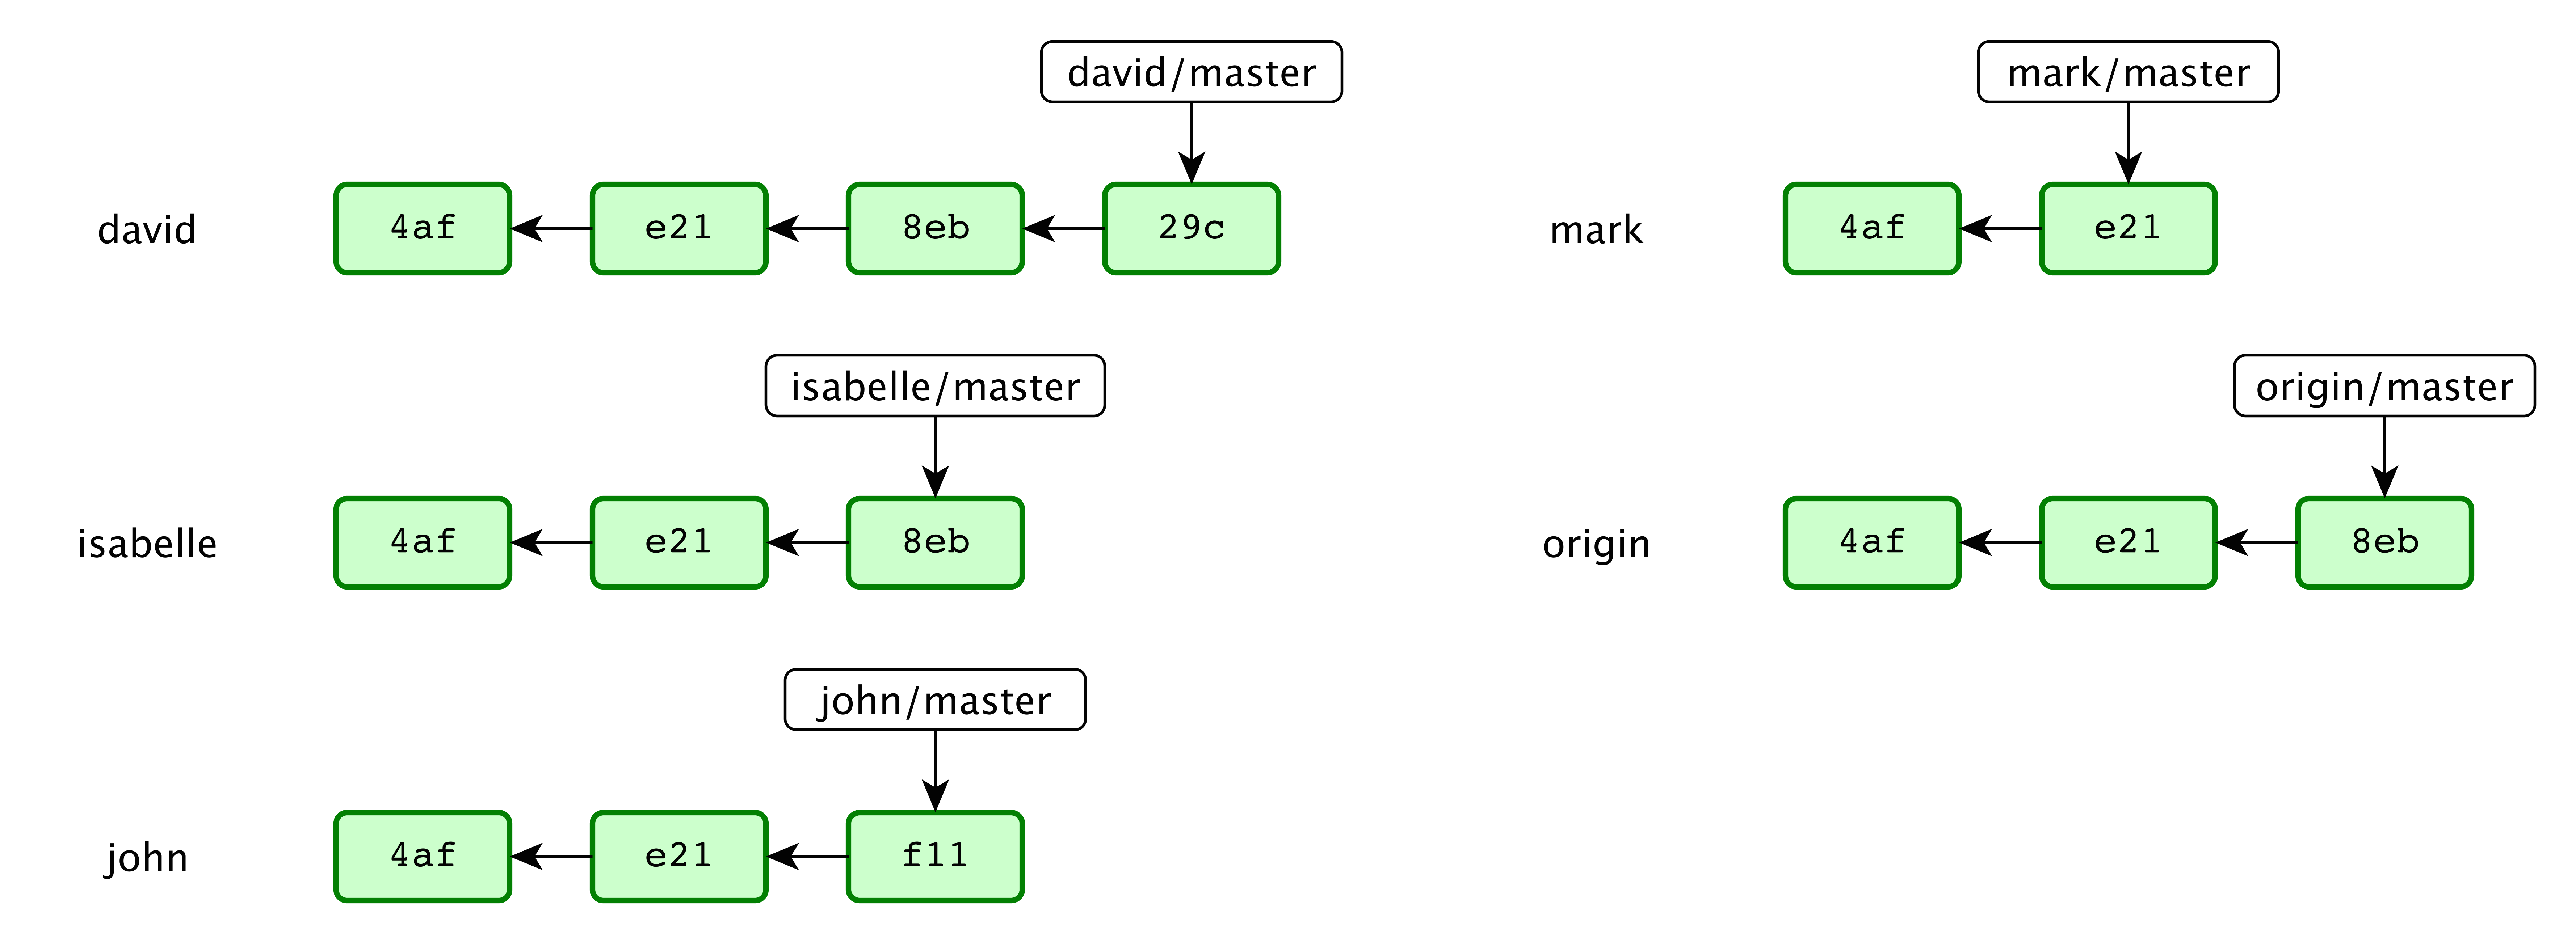
\includegraphics[width=1\textwidth]{commitgraph1}
  \caption{Commit history graph for users in a system}
  \label{fig:commitgraph1}
\end{figure}


\begin{figure}[h!]
  \centering
      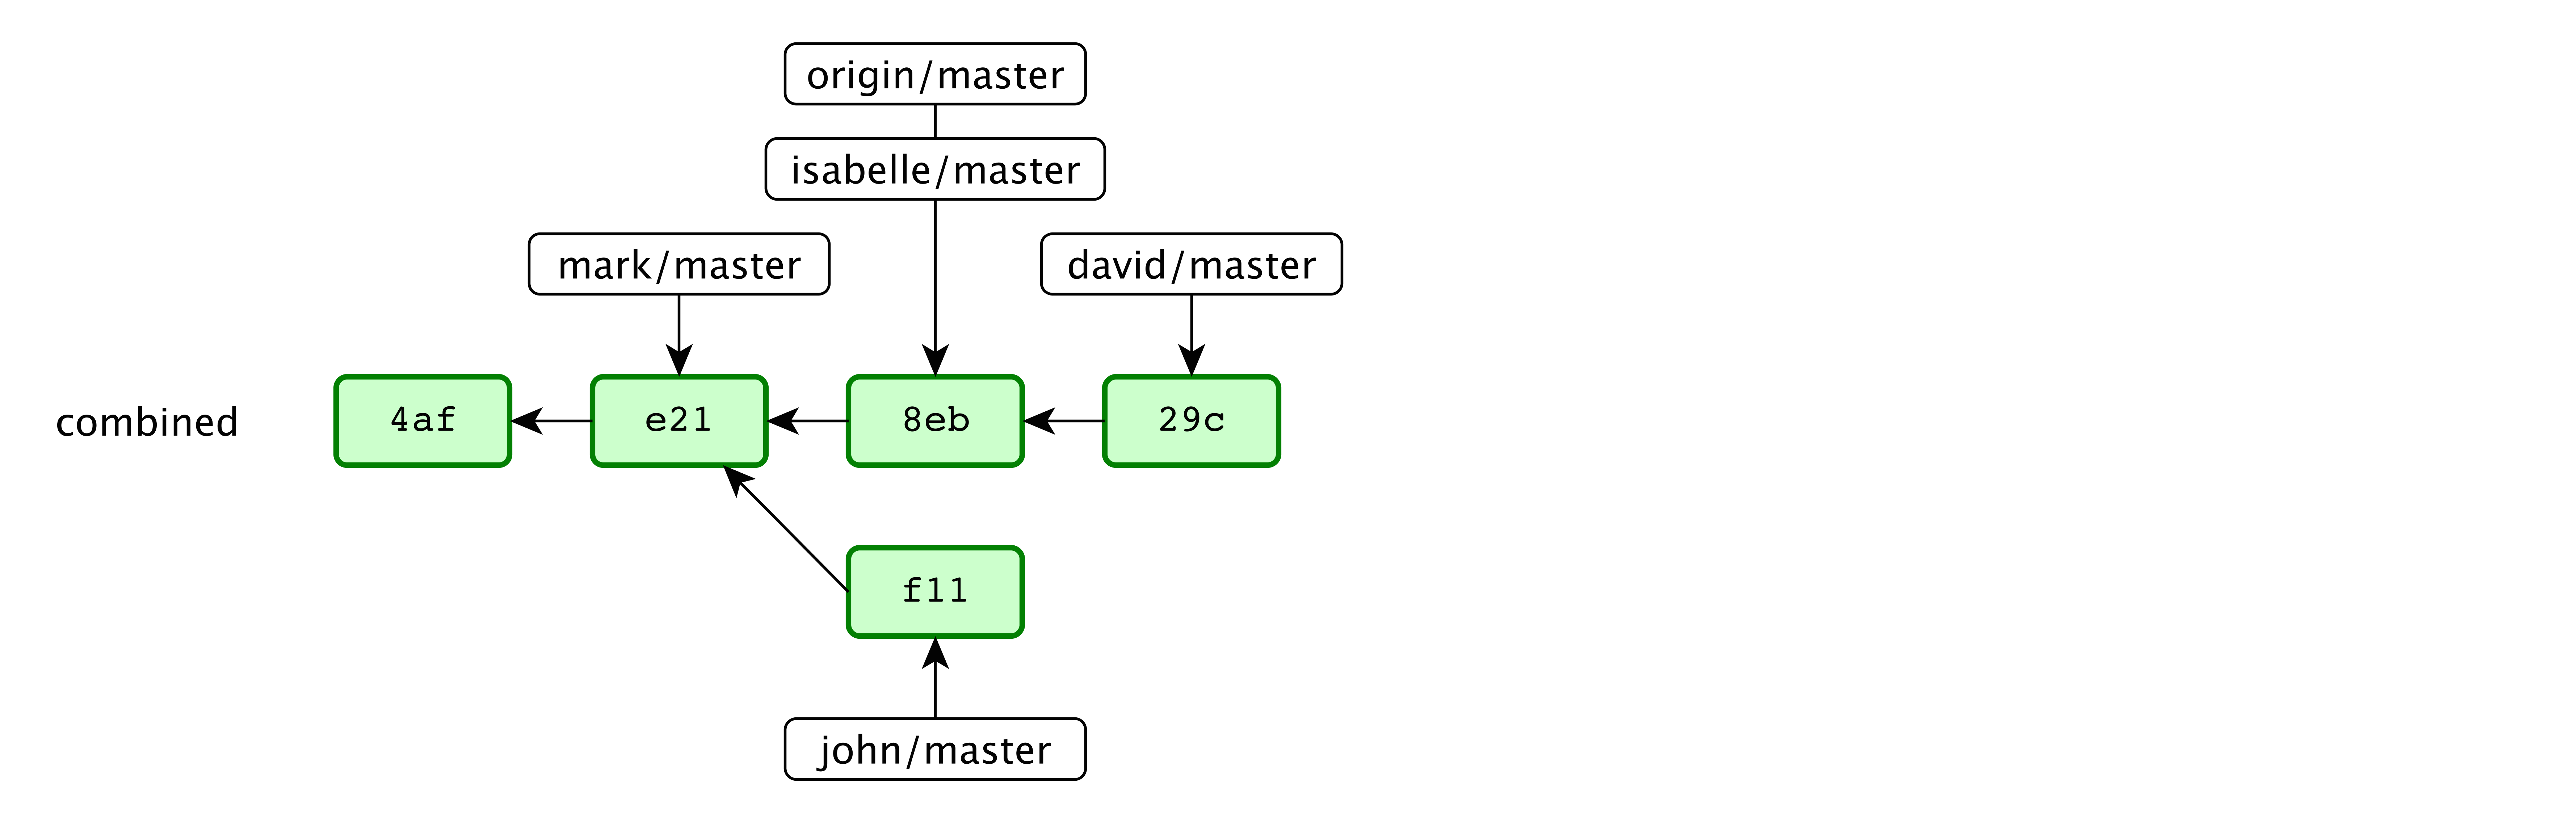
\includegraphics[width=1\textwidth]{commitgraph2}
  \caption{Combined commit history graph}
  \label{fig:commitgraph2}
\end{figure}

From this graph we can deduct the following relationships:

\begin{itemize}


\item Isabelle is $equal$ to the origin. Her local repository is up to date and she has not made any further local commits.
\item David has made a new local commit after his last repository pull and has not pushed it to the origin yet. He is $ahead$ of the origin, with a distance of 1 because he needs to traverse one edge in the graph to reach the commit that the origin is pointing to. David could at this point push his changes to the origin and the origin would simply fast-forward merge, meaning it will add the new commit and point its master branch reference to \texttt{29c}.
\item Mark is $behind$ the origin; he has pulled from the origin when \texttt{e21} was the active commit and has not pulled or made a local commit since.
\item John is in a $fork$, with a distance of 2, as he has also last pulled from the origin at \texttt{e21} but has made a local commit (\texttt{f11}). In the meantime someone (either Isabelle or David, given the commit graph) has made a commit (\texttt{8eb}) and pushed it to the server. If John wanted to push his changes to the server, a merge between \texttt{8eb} and \texttt{f11} would be made and stored in a new commit.

\end{itemize}


The same reference pointers that the example shows for the master branch are also given for all other branches in the system and the calculations behave analogous. If a user has a branch pointer for a branch that isn'tt on the origin, the relationship is given as $local$ $branch$; for a branch that only exists on the origin but not in a users local repository, the relationship is $remote$ $branch$. \\

This awareness feature only deals with locally committed changes and is a useful measure of how up to date local repositories are in relation to the origin. If a user is a $behind$, they should perform a pull. If they are $ahead$, they should push their changes. If they are in a $fork$, it means they started working on a feature while in the meantime someone else pushed their local changes; this case will necessarily result in a merge. $Forks$ will occur often, as the only way to avoid them is if only one user is making a change at the time. A low distance can indicate that fewer changes have been made, while a high distance can indicate a big amount of changes. \\

For each branch in this view, a list of active users is given. If a user has currently checked out a specific branch into their local working tree, it is their "active repository" and it indicates they are working on it. This is very useful to get an overview of what all users are working on, especially if branches have meaningful names (e.g. ticket identifier for feature tickets) and there are many users in a project. \\

A timestamp shows the last time that the user has updated their state via the CloudStudio client and indicates how recent and accurate the provided information is for each user. This way, users do not falsely rely on outdated information.






\section{File Level Awareness}

As the second step in a usual navigation path through the awareness system, the file level view shows awareness information and possible conflicts for all files in a repository and branch. This is achieved by doing a pair-wise comparison of your version of a file with all the version of all users in this branch. Alternatively you can also choose to view differences from the origin's point of view. \\

In its basic form, the file level awareness view compares file checksums to find out whether a file has been modified. If the two file versions that are being compared are not identical, this is presented as a file conflict. It should be noted that non-existing files are treated as empty files for the purpose of this comparison.


\subsection{View as Origin}

If you are viewing from the origin's point of view, a file conflict indicates that the latest version in the remote repository and a user's local file differ; speaking in terms of awareness: all users that are shown up as conflicting have changed their file locally and are probably working on it. If you choose to show uncommitted changes, it will compare the most up to date version of a file from each user's working tree; otherwise it will use the latest locally committed version. \\

This viewpoint provides useful awareness information to see what users are working on what file. If multiple users show up as a file conflict for the same file, they should coordinate their changes early in order to avoid complicated merge conflicts later on.

\subsection{View as Yourself}

Without the "view as origin" option, your local files are compared directly to all other users'. However, a file conflict is less meaningful here: if you have changed a file, all other users will show up as a file conflict because the file checksums differ. More interesting in this case is to enable the "show conflicts" option.

\subsection{Show Conflicts}

With the "show conflicts" option enabled, the comparison does not directly compare the two file versions, but instead does a three-way comparison by taking the nearest common ancestor of both files from the commit history as the baseline. This emulates the same behaviour that Git would do when performing a merge: Git will select a merge base and try to merge files automatically if different portions of the file have been changed. In this three-way comparison, a merge conflict would by definition occur exactly, if in some part either all three files differ, or if only the base file differs. \\

For all the files and users that would show up as file conflicts (without this option enabled), this three-way comparison will additionally look for merge conflicts and mark files that would not pass an automatic merge as content conflict. This is very useful, because when two users are working on a file simultaneously but they are working on different parts, no content conflicts are shown. As soon as they are changing the same portions of a file and Git would have trouble merging the files at a later point, a content conflict is displayed. This helps catching merge conflicts very early on and users can arrange their work and take countermeasures before the merge overhead becomes bigger.

\subsection{Compare to Other Branches}

The same functionality can not only be used to show branch internal awareness and conflict information---by specifying a different comparison branch, your (or the origin's) files from your selected branch are compared with all other users' in the specified branch. \\

Let's say you are working on the master branch and someone else is called on a feature branch $iss53$ that will have to be merged into the master branch at a later point in time. \\

By selecting branch comparison with $iss53$ from the viewpoint of the master branch, you can see file and content conflicts that will occur when merging your local master branch state with each other user's $iss53$ branch state. Likewise, by comparing with the master branch from $iss53$'s point of view, the comparison will be made between your files from the master branch with all other users' files in the $iss53$ branch. \\

In the same manner, the comparison functions with the "view as origin" option enabled: instead of your files from the selected branch, the files from the origin will be compared.

\subsection{Filters}

You can choose to filter your view by only selecting a subset of the users in a project. If the number of users is really big, this helps narrow down your search and display only information relevant to you. \\

It is also possible to filter files by the severity of conflicts. Selecting "content conflicts" only shows files and users with a conflict type of "content conflicts", "file conflicts" shows both file and content conflicts, an no filter also shows users where the files are identical.

\subsection{Grouping}

Folders have a grouping mechanism that add up the containing conflicts. If a user contains at least one content conflict, it will be marked as a folder containing content conflicts and the users responsible for it will be listed. Likewise file conflicts propagate their conflict type up to the containing folders.

\subsection{Uncommitted vs. Committed Files}

As already mentioned above, you can always select to work either with locally committed files or uncommitted files directly from the active working tree from all users. Working with uncommitted files has the advantage of always have the latest version of all files, while you are running into the risk that these changes may not be final or only experimental and will never make it into an actual commit. Viewing committed files is more safe in this regard, but may not show very recent changes.







\section{Content Level Awareness}




The content level awareness view allows you to compare two versions of a file side-by-side. \\

In non-conflict mode, files are compared side-by-side directly and insertions, deletions and modifications are highlighted. \\

In the conflict mode, the closest common ancestor in the commit history is taken as a base file for a three-way comparison. The comparison is done using the diff3 algorithm that is also used by Git to internally merge files automatically. Sections of the file are matched into blocks; if a block has been changed in all three files or only in the base file, a conflict occurs, because a three-way merge could not automatically decide how to merge these blocks together. These conflicts are highlighted in red, while normal modifications that would be merged automatically by Git are shown in light blue. \\

The content awareness view allows you to toggle the options to "show uncommitted files", "show conflicts" and "view as origin" directly in place.







